\section{Signal/background comparisons}
\label{app:SignalBackgroundComparison}

\subsection{BDT input variables}
\label{subapp:SOVERB_BDTInputVars}
Figures \ref{fig:SOVERB_BDTInputs_Hp} (Figure \ref{fig:SOVERB_BDTInputs_Hp}) compare the shape of the variables included in the BDT for all $H^{+}$ ($W'$) signal masses and background.

\begin{figure}[H]
    \subfloat[HT\_jets] {
        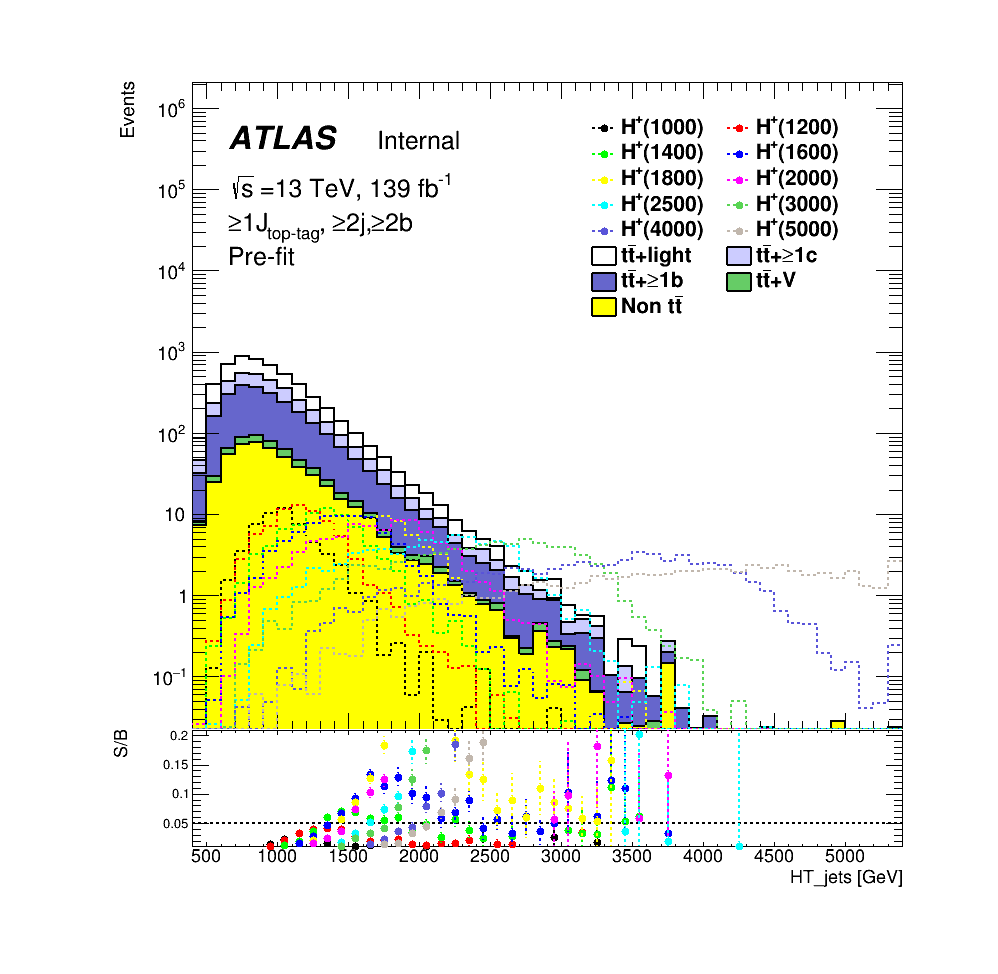
\includegraphics[width=0.50\textwidth]{images/SigBkgComparison/SOVERB_HTjets_beforeRW_geq1tgeq2jgeq2b.png}
        \label{fig:SOVERB_HT_jets}
    }
    \subfloat[LeadingJet\_pt] {
        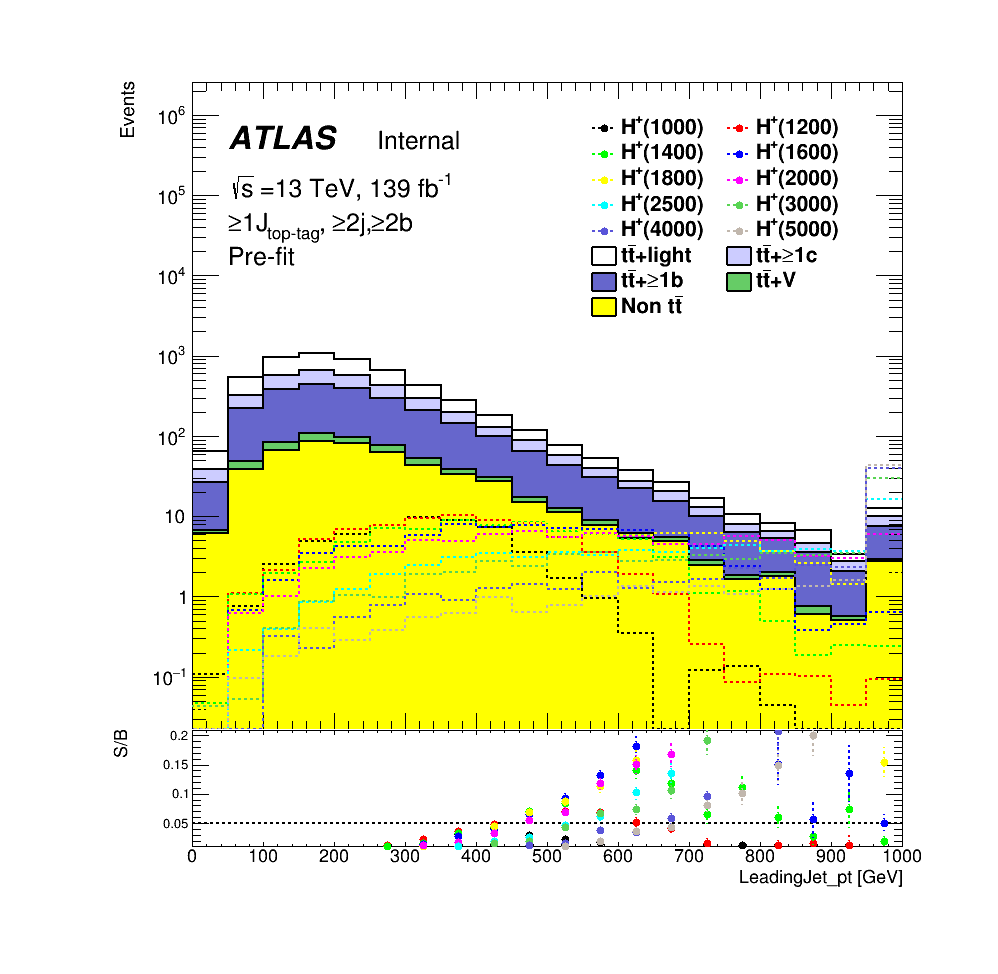
\includegraphics[width=0.50\textwidth]{images/SigBkgComparison/SOVERB_LeadingJet_pt_beforeRW_geq1tgeq2jgeq2b.png}
        \label{fig:SOVERB_LeadingJet_pt}
    }
\end{figure}
\begin{figure}[H]
    \addtocounter{figure}{-1}
    \subfloat[Centrality\_all] {
        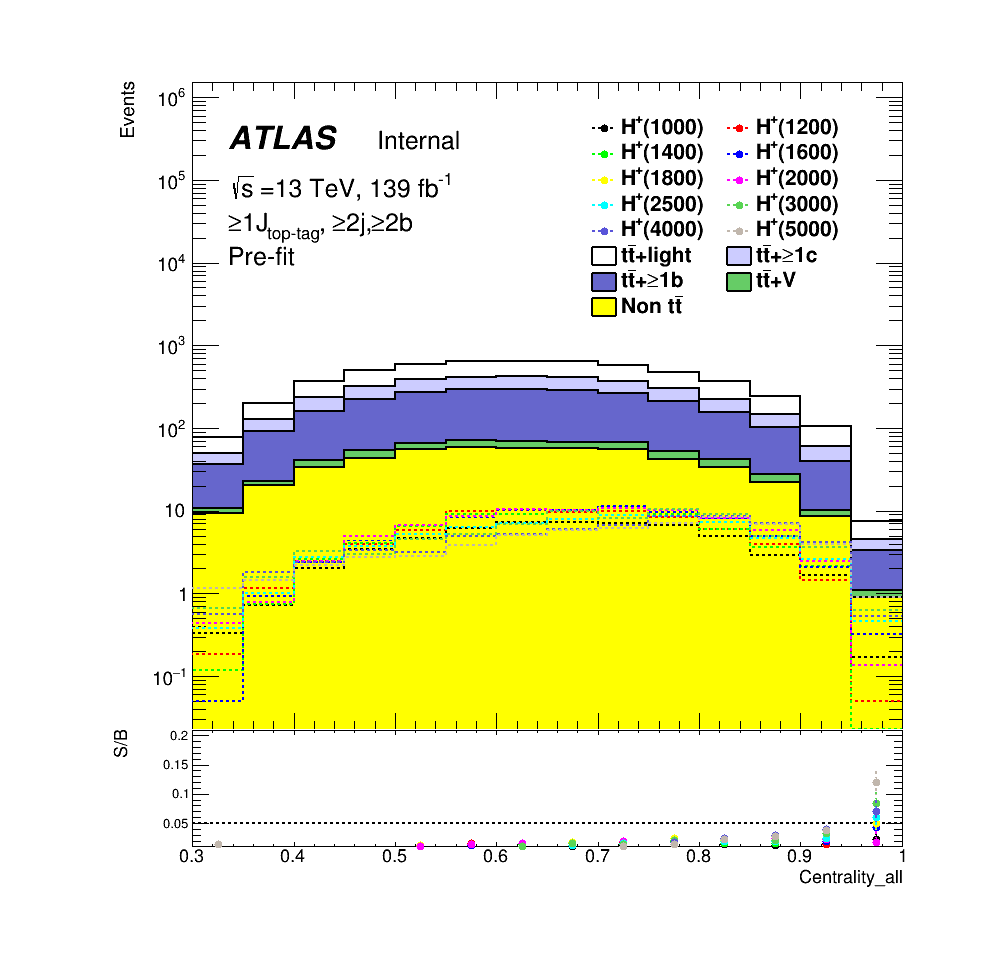
\includegraphics[width=0.50\textwidth]{images/SigBkgComparison/SOVERB_Centrality_all_beforeRW_geq1tgeq2jgeq2b.png}
        \label{fig:SOVERB_Centrality_all}
    }
    \subfloat[H1\_all] {
        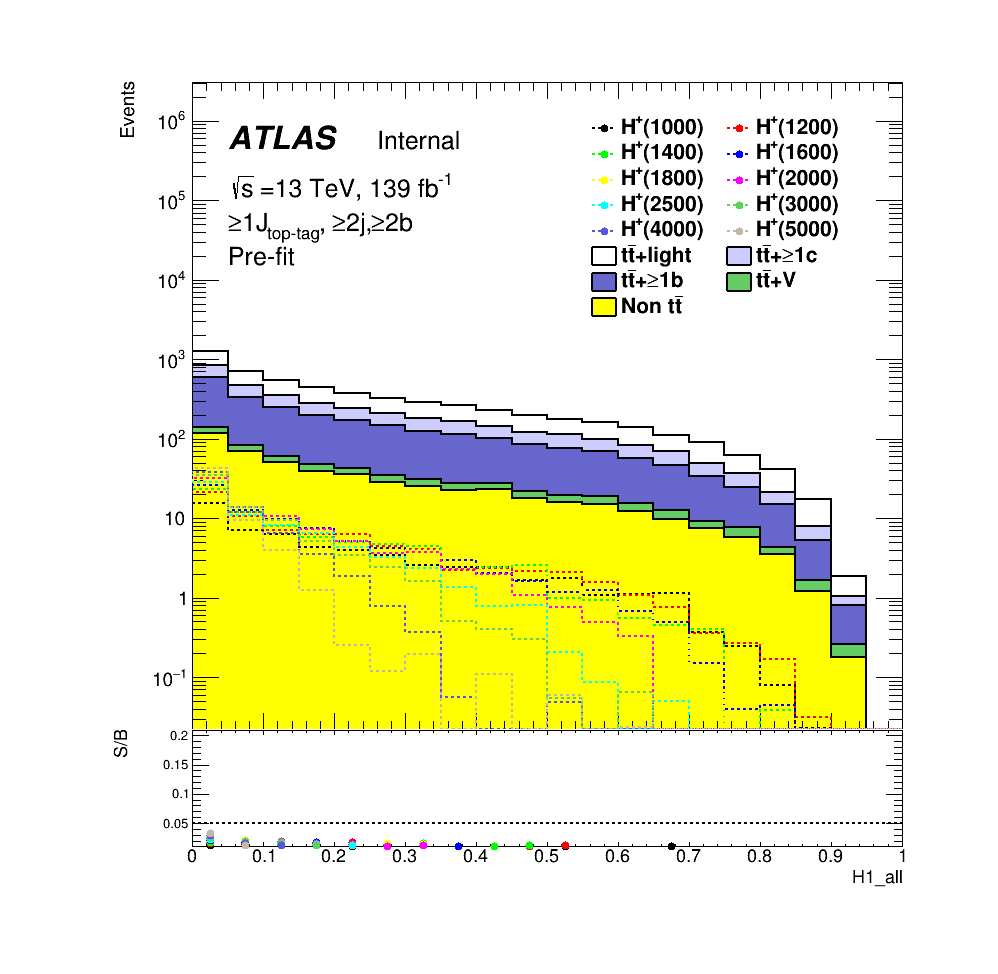
\includegraphics[width=0.50\textwidth]{images/SigBkgComparison/SOVERB_H1_all_beforeRW_geq1tgeq2jgeq2b.png}
        \label{fig:SOVERB_H1_all}
    }
\end{figure}
\begin{figure}[H]
    \addtocounter{figure}{-1}
    \subfloat[Mbb\_MaxPt] {
        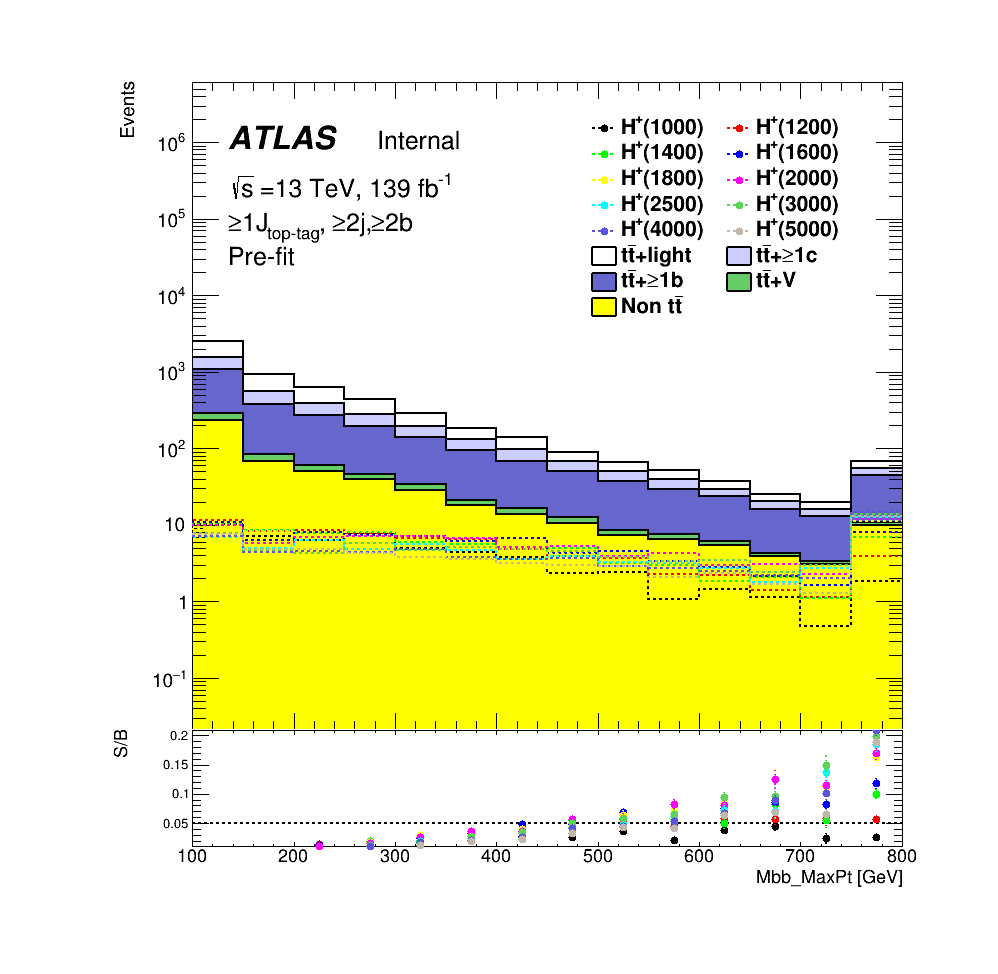
\includegraphics[width=0.50\textwidth]{images/SigBkgComparison/SOVERB_Mbb_MaxPt_beforeRW_geq1tgeq2jgeq2b.png}
        \label{fig:SOVERB_Mbb_MaxPt}
    }
    \subfloat[Mjjj\_MaxPt] {
        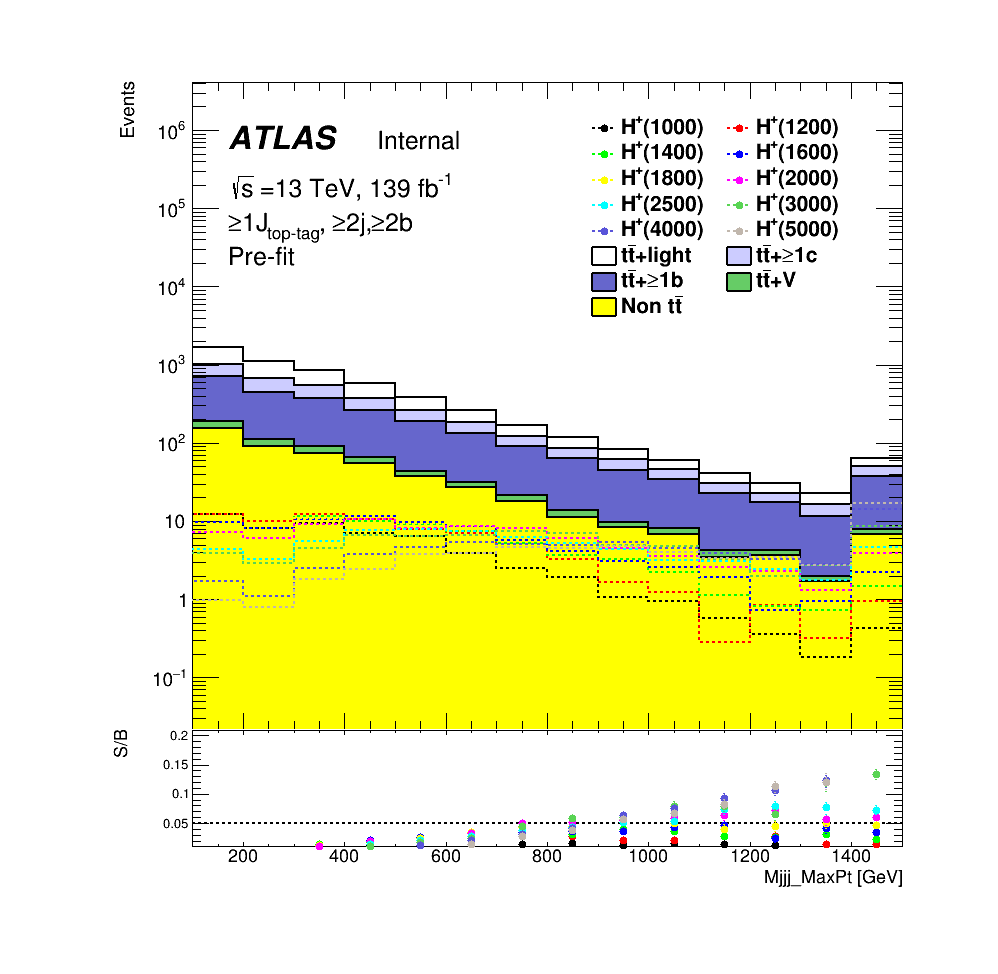
\includegraphics[width=0.50\textwidth]{images/SigBkgComparison/SOVERB_Mjjj_MaxPt_beforeRW_geq1tgeq2jgeq2b.png}
        \label{fig:SOVERB_Mjjj_MaxPt}
    }
\end{figure}
\begin{figure}[H]
    \addtocounter{figure}{-1}
    \subfloat[Muu\_MindR] {
        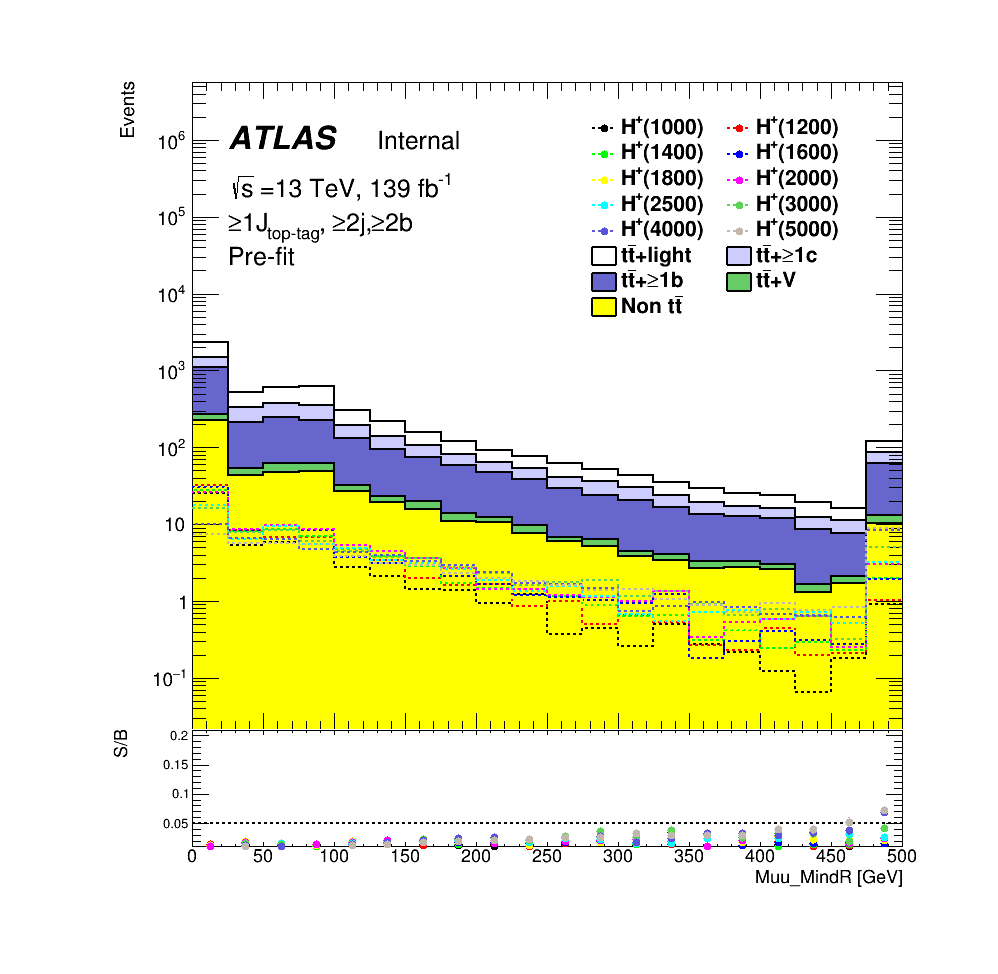
\includegraphics[width=0.50\textwidth]{images/SigBkgComparison/SOVERB_Muu_MindR_beforeRW_geq1tgeq2jgeq2b.png}
        \label{fig:SOVERB_Muu_MindR}
    }
    \subfloat[dRbb\_avg] {
        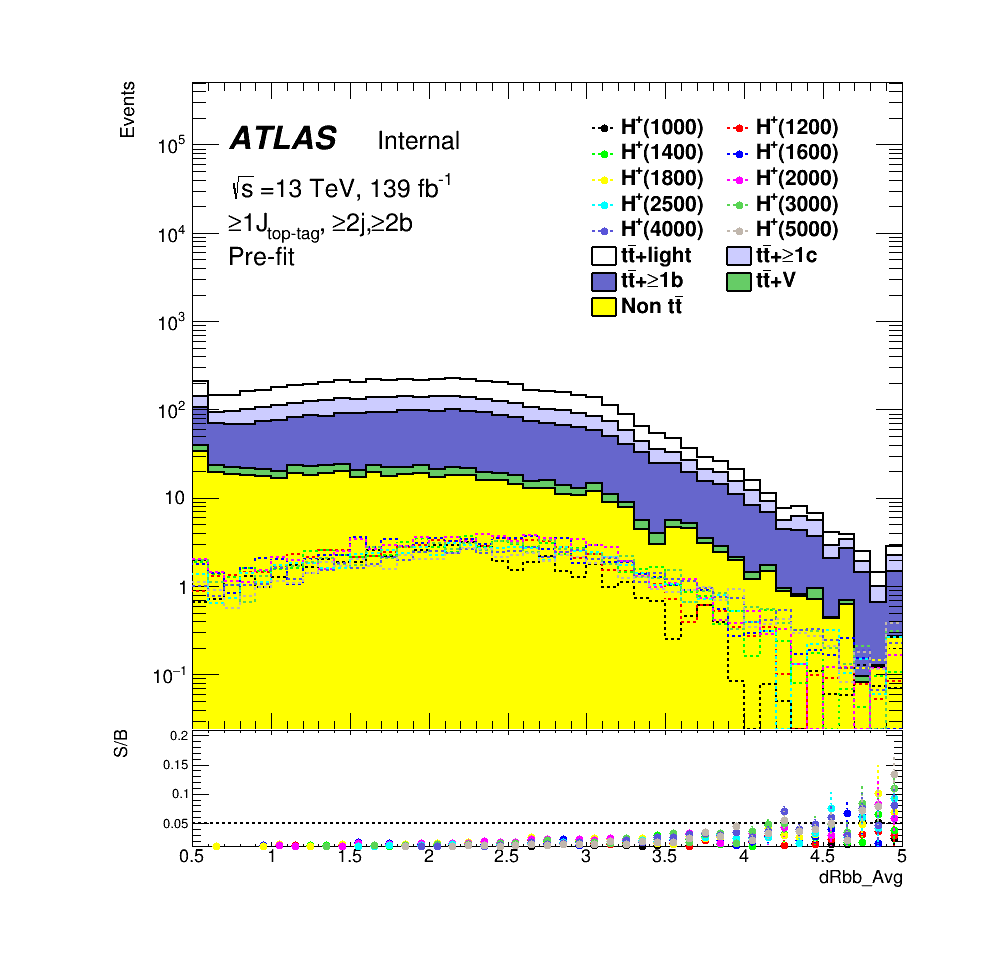
\includegraphics[width=0.50\textwidth]{images/SigBkgComparison/SOVERB_dRbb_avg_beforeRW_geq1tgeq2jgeq2b.png}
        \label{fig:SOVERB_dRbb_avg}
    }
\end{figure}
\begin{figure}[H]
    \addtocounter{figure}{-1}
    \subfloat[dRlepbb\_MindR] {
        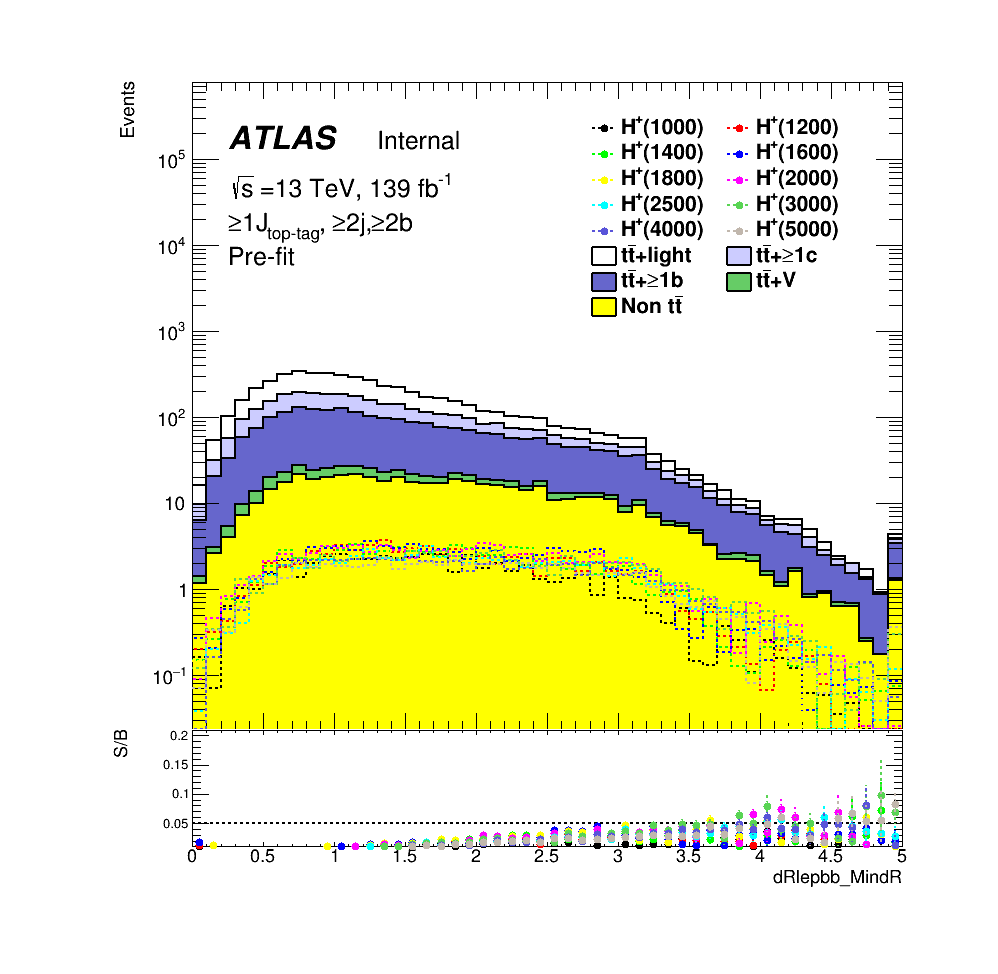
\includegraphics[width=0.50\textwidth]{images/SigBkgComparison/SOVERB_dRlepbb_MindR_beforeRW_geq1tgeq2jgeq2b.png}
        \label{fig:SOVERB_dRlepbb_MindR}
    }
    \subfloat[LeadingTop\_m] {
        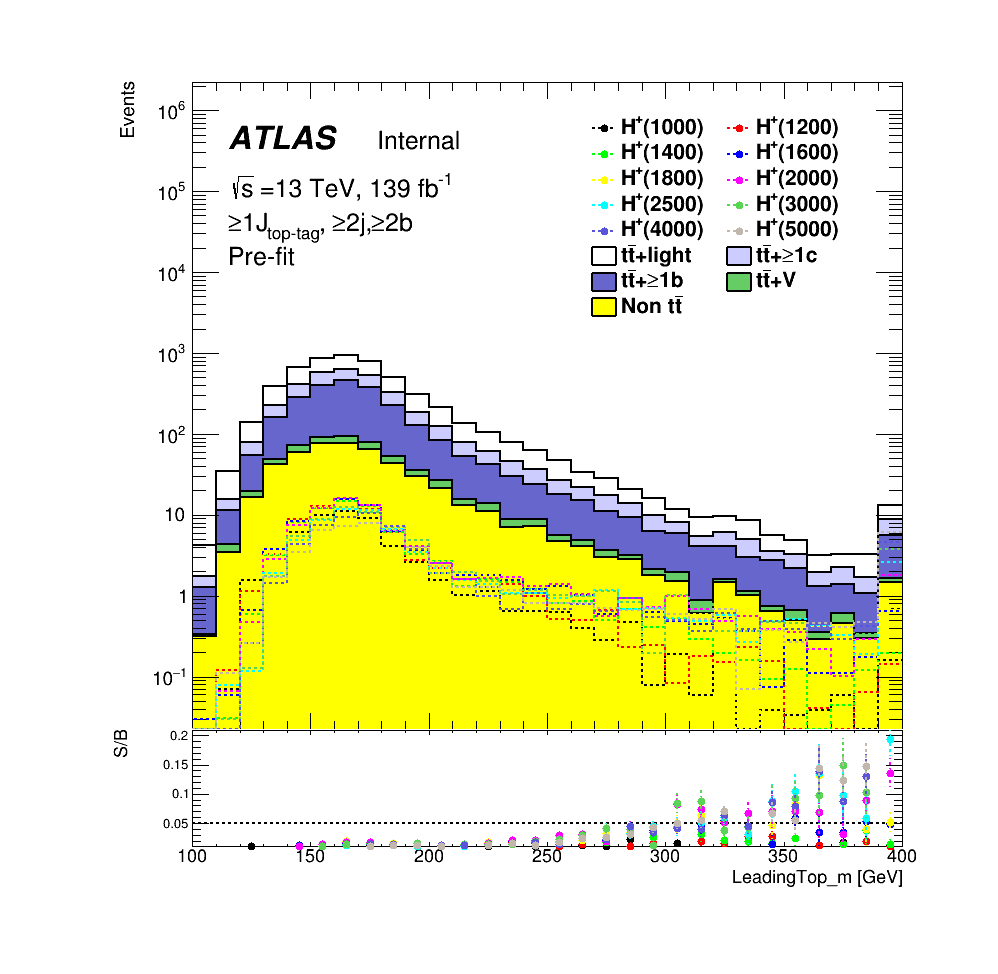
\includegraphics[width=0.50\textwidth]{images/SigBkgComparison/SOVERB_LeadingTop_mass_beforeRW_geq1tgeq2jgeq2b.png}
        \label{fig:SOVERB_LeadingTop_mass}
    }
\end{figure}
\begin{figure}[H]
    \addtocounter{figure}{-1}
    \subfloat[LeadingTop\_pt] {
        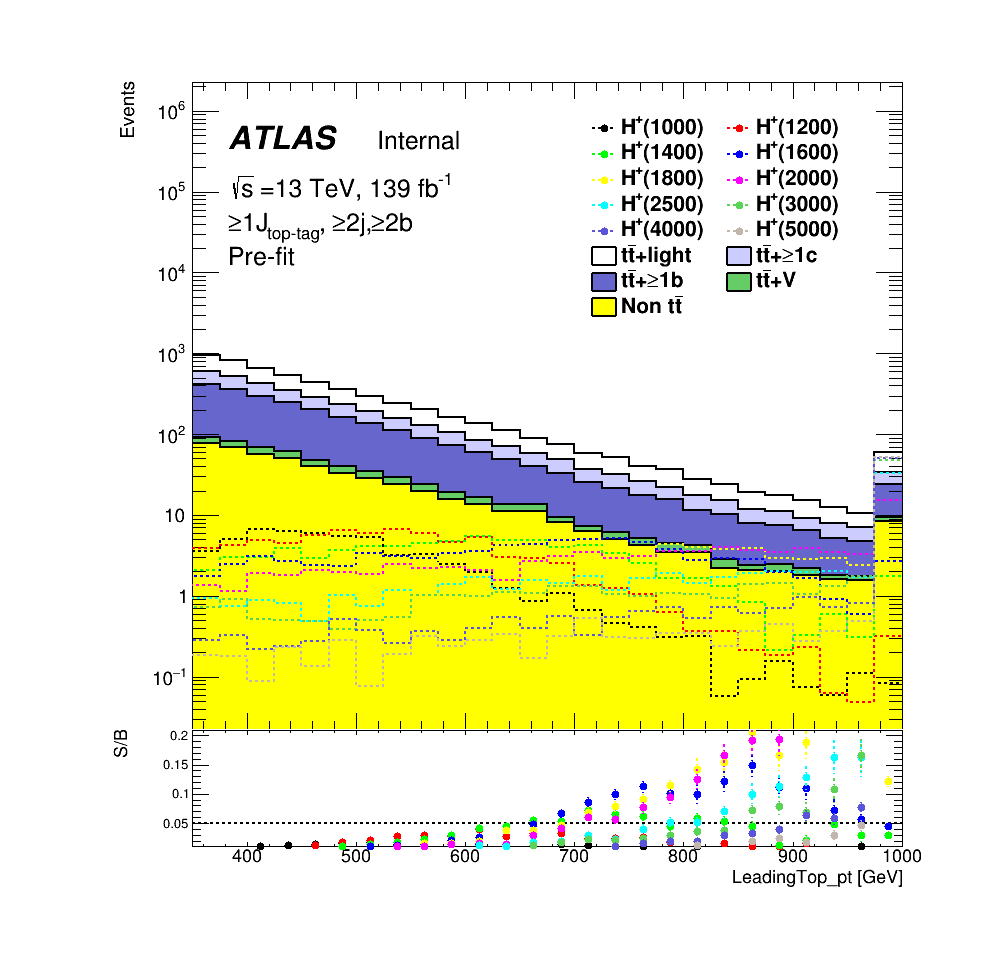
\includegraphics[width=0.50\textwidth]{images/SigBkgComparison/SOVERB_LeadingTop_pt_beforeRW_geq1tgeq2jgeq2b.png}
        \label{fig:SOVERB_LeadingTop_pt}
    }
    \subfloat[M\_tb] {
        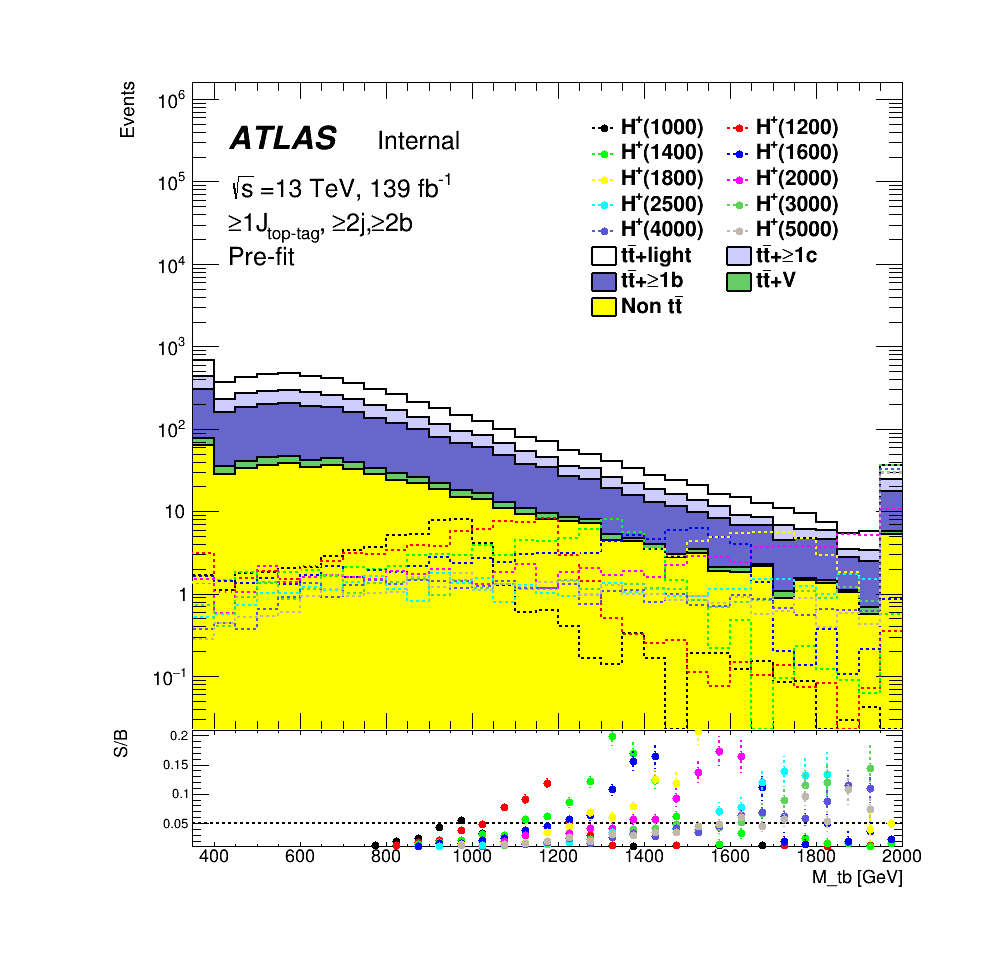
\includegraphics[width=0.50\textwidth]{images/SigBkgComparison/SOVERB_tb_mass_beforeRW_geq1tgeq2jgeq2b.png}
        \label{fig:SOVERB_tb_mass}
    }
\end{figure}
\begin{figure}[H]
    \addtocounter{figure}{-1}
    \subfloat[Pt\_tb] {
        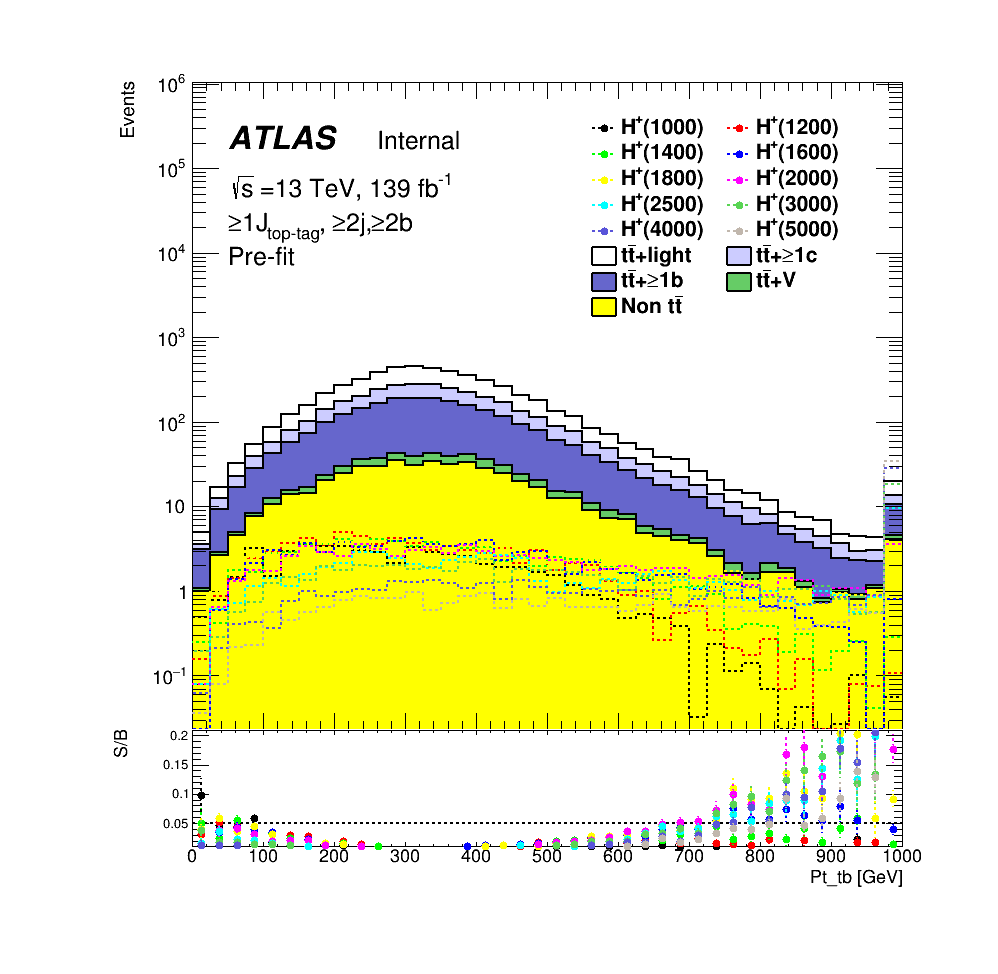
\includegraphics[width=0.50\textwidth]{images/SigBkgComparison/SOVERB_tb_pt_beforeRW_geq1tgeq2jgeq2b.png}
        \label{fig:SOVERB_tb_pt}
    }
    \subfloat[PtAsymm\_tb] {
        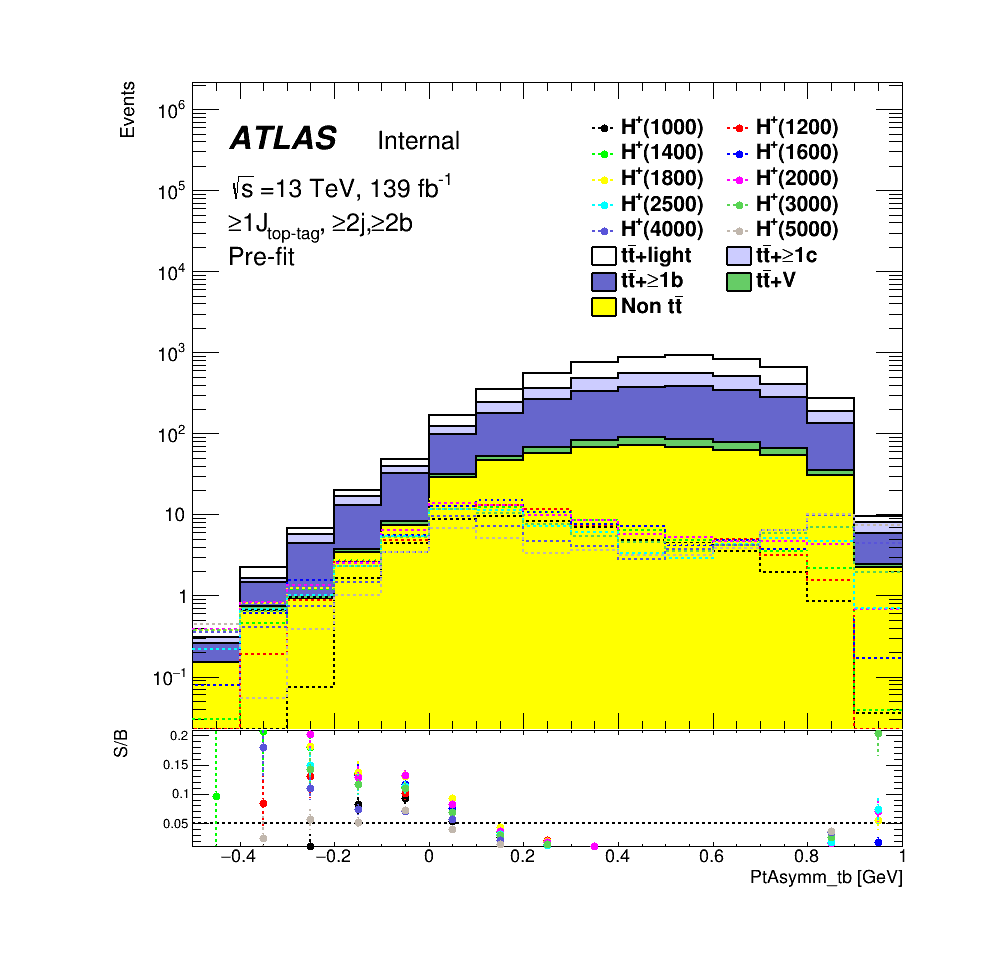
\includegraphics[width=0.50\textwidth]{images/SigBkgComparison/SOVERB_tb_ptAsymm_beforeRW_geq1tgeq2jgeq2b.png}
        \label{fig:SOVERB_tb_ptAsymm}
    }
    \caption{Comparison of the kinematic variables included in the BDT in the SR for the various $H^{+}$ signal masses between signal and background.}
    \label{fig:SOVERB_BDTInputs_Hp}
\end{figure}





\subsection{BDT outputs}
\label{subapp:SOVERB_BDTOutput}
\subsection{Comparison using distributions with binning }